\fontsize{14}{15}\selectfont
\setcounter{secnumdepth}{5}

\section{OBJETIVO GENERAL}
Evaluar la adaptación de las técnicas existentes de extracción de palabras clave en el contexto de textos cortos formales y semi-informales en español.

\section{OBJETIVOS ESPECÍFICOS}
\begin{itemize}
  \item Caracterizar el conjunto de técnicas de extracción de palabras clave más representativas o adaptables al idioma español.
  \item Implementar una adaptación de los 3 métodos más relevantes arrojados en el análisis de técnicas encontradas.
  \item Evaluar la aplicación de los métodos para determinar cuáles son sus características de desempeño, frente a textos cortos formales y semi-informales en español, en el dominio específico de los registros de llamadas de usuarios del servicio de Mentes Colectivas de la Pontificia Universidad Javeriana.
\end{itemize}


\section{FASES DE DESARROLLO}
Para el desarrollo del Proyecto en general, se aplicará la metodología Scrum, planteando Spritns de dos semanas, durante las cuales se establecerán diferentes tareas. \par
Para lo que corresponde a la aplicación específica sobre los registros de llamadas de los usuarios del servicio de Mentes Colectivas, se aplicará la metodología CRISP-DM (Cross-Industry Standard Process for Data Mining). 

\subsection{Metodología CRISP-DM}
La metodología CRISP-DM es una de las metodologías más utilizadas en proyectos de minería de datos; dicha metodología es representada como un ciclo, en el cual se ejecu-tan 6 fases que no necesariamente son dependientes la una de la otra, ya que se permite (en algunas fases) realizar retornos a fases anteriores, permitiendo así, generar mejores resultados sobre el proyecto. A continuación, se presenta una ilustración del ciclo de minería de datos según CRISP-DM:

\begin{figure}[h]
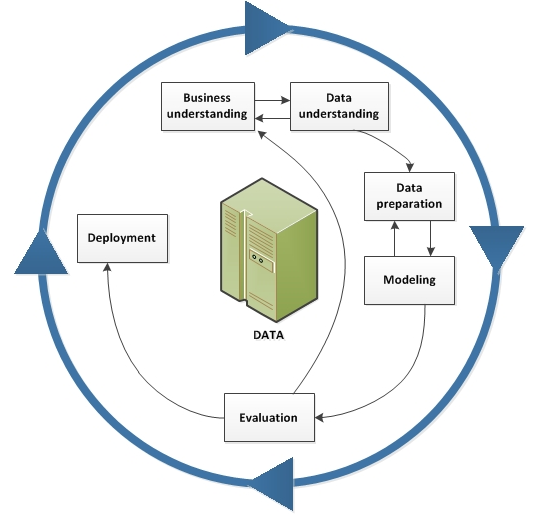
\includegraphics[scale=0.7]{Documento Trabajo de Grado/figures/CicloDeVidaCRISPDM.png}
\centering
\caption{Ciclo de Vida CRISP-DM}
\centering
\end{figure}

La metodología CRISP-DM está compuesta por las fases enumeradas en las siguientes secciones.

\subsubsection{Entendimiento del Negocio}
Esta primera fase busca 
\subsubsection{Entendimiento de los Datos}
\subsubsection{Preparación de los Datos}
\subsubsection{Modelamiento}
\subsubsection{Evaluación}
\subsubsection{Despliegue}


\subsection{Metodología SCRUM}